\section{Nouveau Programme}

\subsection{Introduction}

Le nouveau programme, réalisé tardivement, accélères énormément les temps de calculs. Une simulation réalisé avec l'ancien programme à mit plus d'une heure alors que celle lancé avec le nouveau a durée que quelques secondes.

Grâce à cela, il nous est maintenant possible de dimensionner une installation beaucoup plus importante est plus cohérente. En effet, nous pouvons maintenant modéliser l'évolution de la température à travers de nombreux tubes et donc imaginer un serpentin avec une section d'entrée faible, conditionné sous forme d'un cube.

\subsection{Principe logique}

Le problème étant la taille de la matrice de résolution, nous avons segmenté sa taille. Nous résolvons l'équation pour un nombre d'élément définit par la variable $"Nb\_iteration\_espace"$.

 Ainsi, si nous mettons un élément, nous calculons ses températures en résolvants une matrice carré de taille Nc+1. Pour faire cela, nous faisons le calcule pour un élément, nous écrivons le résultat et nous stockons les températures dans une matrice. 
 
 Après avoir réalisé cela sur le stockage et de-stockage, nous passons à un autre élément en récupérant les valeurs de la résolution précédente. Ainsi, nous complétons l'échangeur au lieu de tous recalculer avec une énorme matrice. Nous devons bien noté que nous stockons la température de l'air de sortie de l'élément à tous les pas de temps, dans un vecteur, car l'élément suivant est essentiellement dépendant de la température de l'air de l'élément précédant à tous les pas de temps. 

Pour clarifier cette explication nous présentons l'organigramme dans la section qui suit.

\newpage
\subsection{Organigramme}

\begin{figure}[!h]
\centering
\caption{Organigramme du nouveau programme : partie 1}
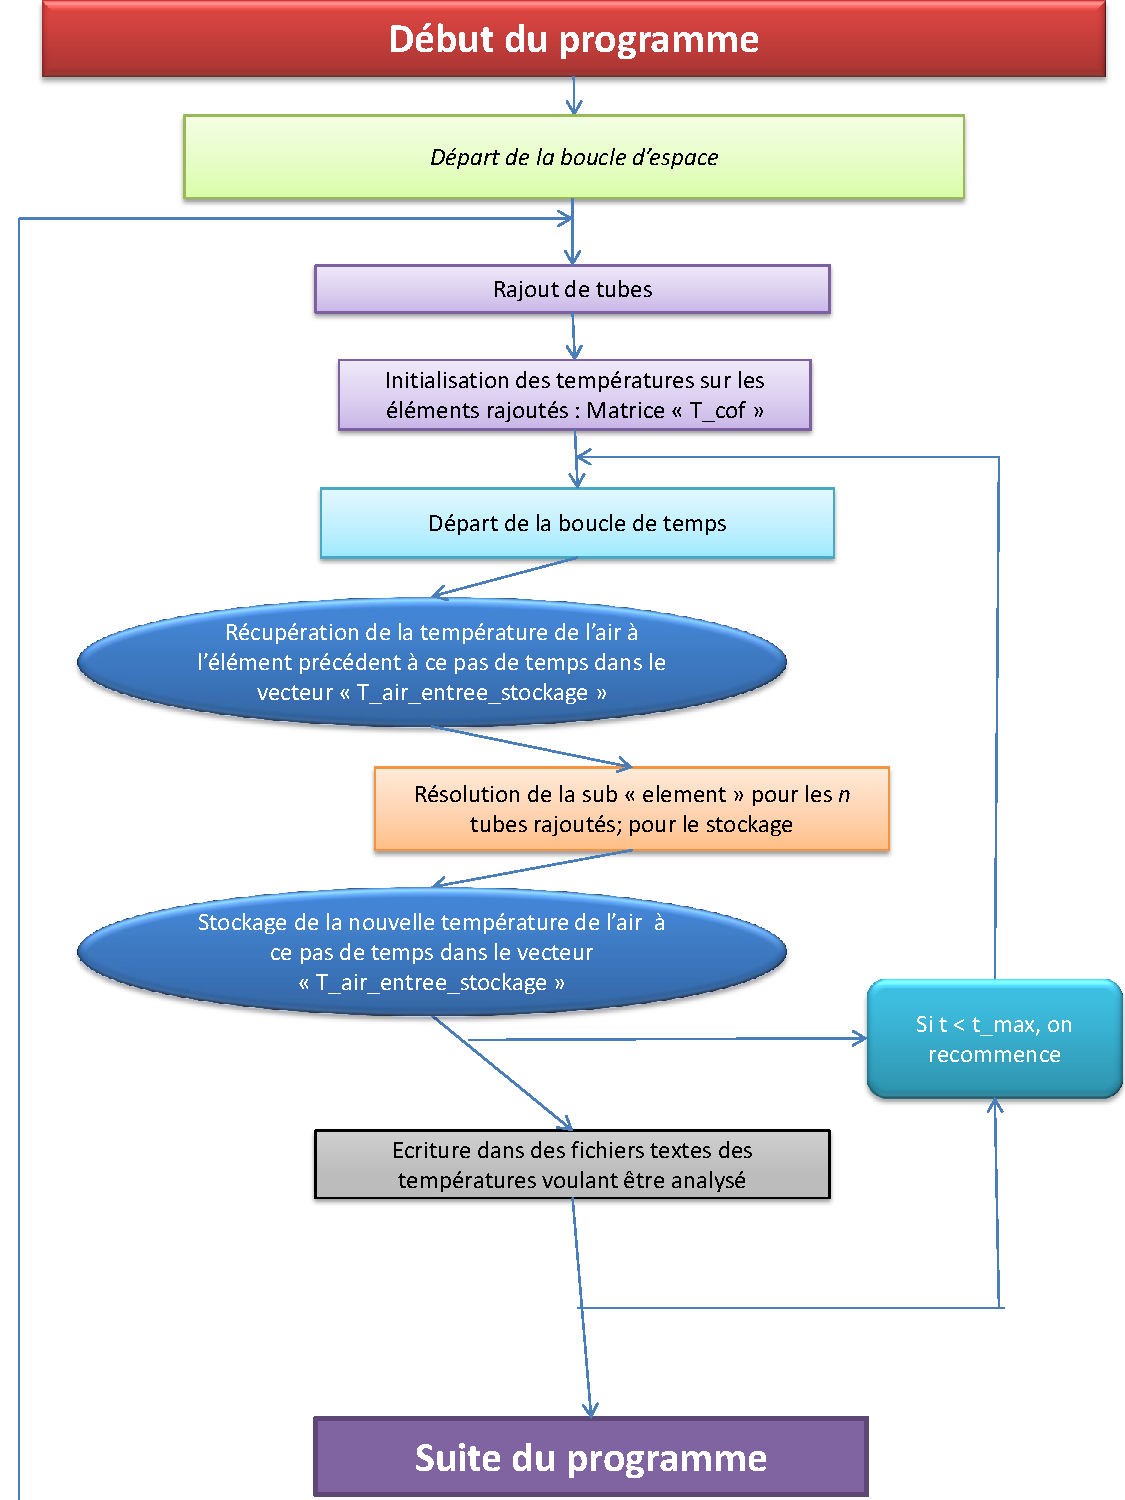
\includegraphics[scale=0.8]{PHOTO/Organigramme_dernier_prog_1.pdf}
\label{dernier_prog_1}
\end{figure}



\begin{figure}[!h]
\centering

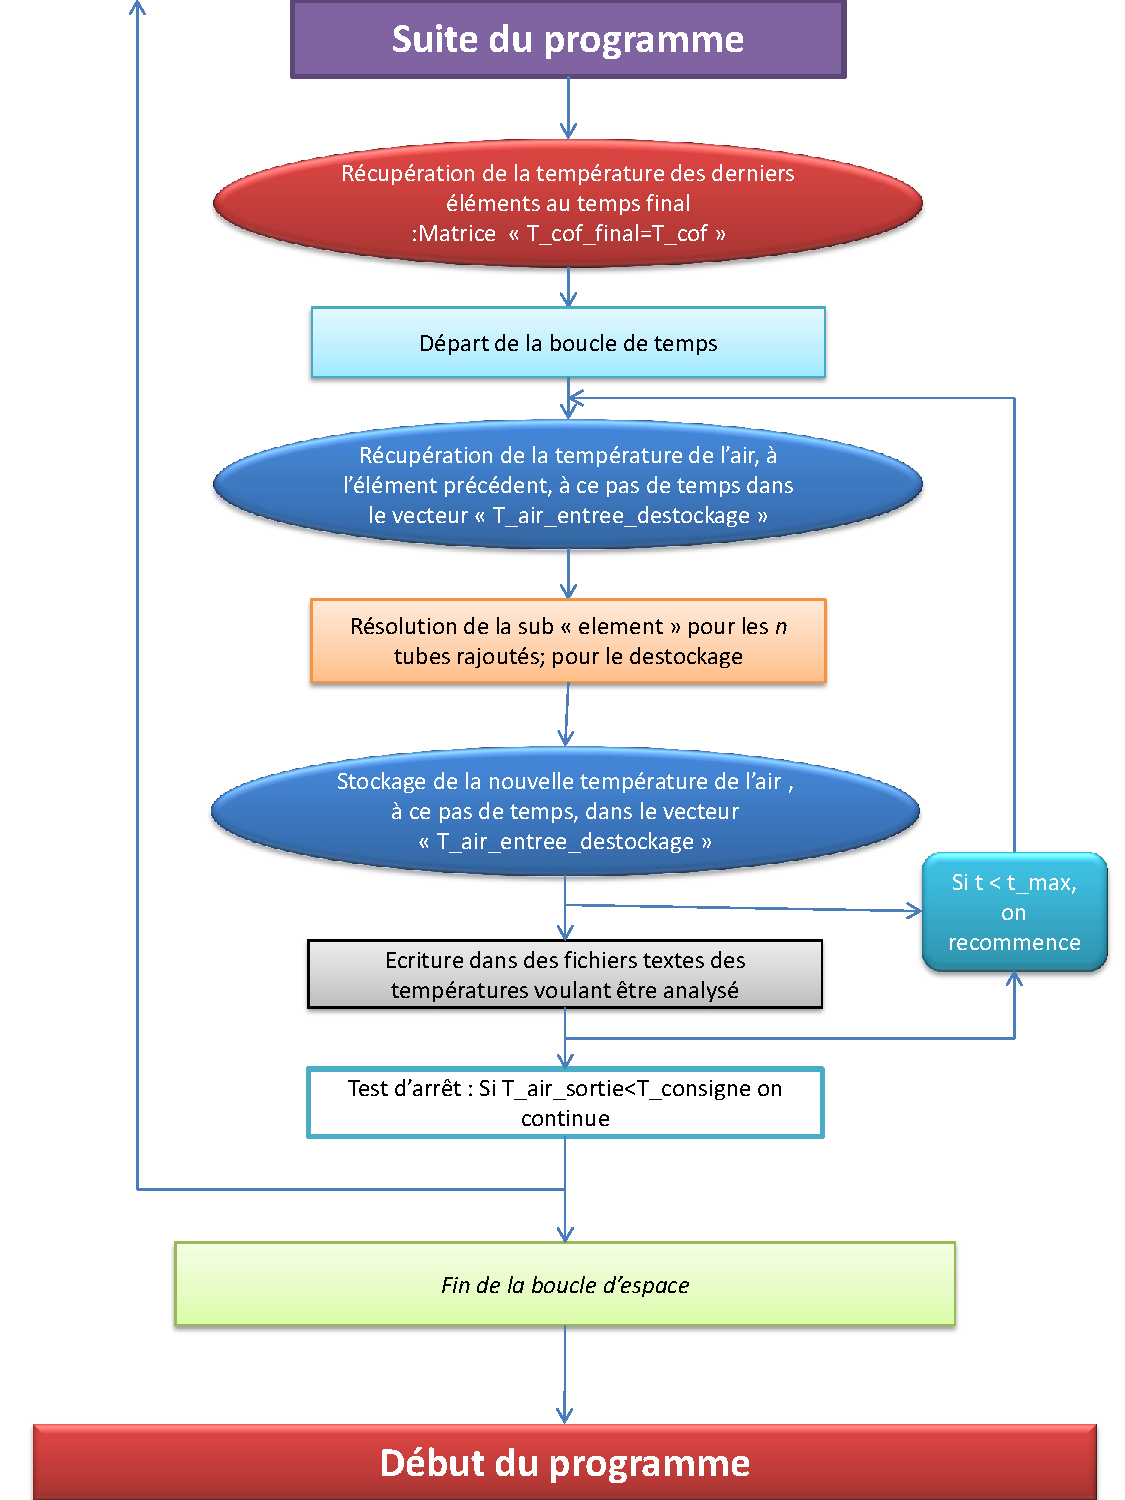
\includegraphics[scale=0.8]{PHOTO/Organigramme_dernier_prog_2.pdf}
\label{dernier_prog_2}
\caption{Organigramme du nouveau programme : partie 2}
\end{figure}
\clearpage




\subsection{Critère d'arrêt}

Nous avons uniquement deux tests d'arrêts sur la version actuelle. L'un permet d'arrêter les itérations sur l'espace lorsque l'on atteint la Température de consigne lors du déstockage. Le deuxième est indirect. La boucle qui rajoute les tubes stop lorsque l'on atteint la valeur de la variable $"Nb\_boucle\_rajout\_tube"$, fixé par l'utilisateur. Nous remarquons indirectement que la multiplication du nombre de tube rajouté, sur chaque pas de la boucle, avec l'indice du pas, donne le nombre de tube sur la hauteur.

Nous fixons donc le nombre de tube par la formule suivante :

\begin{equation}
Nb_tubes=Nb\_boucle\_rajout\_tube * Nb\_iteration\_espace
\end{equation}

\subsection{Remarque}

La variable $"Nb\_iteration\_espace"$ doit être la plus petit possible pour accéléré la vitesse de calcul. Aucun bug notable a été remarqué pour une valeur de 1 et donc ce nombre est conseillé. \\
 
Les tailles de matrice sont les suivantes : 
\begin{itemize}
\item $T\_cof = (Nc+1)Nb\_iteration\_espace$
\item $T\_cof\_final = (Nc+1)Nb\_iteration\_espace$
\item $T\_air\_entree\_stockage = Nb\_iteration\_temps$
\item $T\_air\_entree\_destockage = Nb\_iteration\_temps$
\item Matrice de résolution A : $A = ((Nc+1)Nb\_iteration\_espace) \times ((Nc+1)Nb\_iteration\_espace)$\\

\end{itemize}


Cette astuce pour accéléré drastique-ment la vitesse de calcule numérique a été pensé et réalisé la veille de la date butoir. 
Ainsi, nous n'avons pas eu le temps nécessaire pour perfectionner les détailles et lancer une simulation pour un installation réelle. Cependant, la version actuelle reste fonctionnel et nous présenterons les nouveaux résultats obtenus lors de la soutenance oral.


